\documentclass[a4paper,11pt]{article}

\usepackage[margin=2.3cm]{geometry}
\usepackage{amsmath,amssymb,bm}
\usepackage{booktabs}
\usepackage{longtable}
\usepackage{graphicx}
\usepackage{xcolor}
\usepackage{listings}
\usepackage{hyperref}
\usepackage{float}
\usepackage{caption}
\usepackage{enumitem}
\usepackage{tikz}
\usetikzlibrary{positioning}
\usepackage{fancyhdr}

\hypersetup{colorlinks=true,linkcolor=blue,urlcolor=blue}
\pagestyle{fancy}
\setlength{\headheight}{14pt}
\fancyhf{}
\lhead{Vase Reconstruction}
\rhead{\thepage}

\definecolor{codegray}{RGB}{245,245,245}
\lstset{
  backgroundcolor=\color{codegray},
  basicstyle=\ttfamily\small,
  breaklines=true,
  columns=fullflexible,
  frame=single,
  numbers=left,
  numberstyle=\tiny\color{gray},
  keepspaces=true
}

\newcommand{\figplaceholder}[3][0.88\textwidth]{%
  \begin{figure}[H]
    \centering
    \IfFileExists{#2}{%
      \includegraphics[width=#1]{#2}%
    }{%
      \begin{tikzpicture}
        \draw[dashed,gray] (0,0) rectangle (12,5.5);
        \node[align=center,gray] at (6,2.75)
          {Result figure placeholder\\[2mm]\texttt{#2}};
      \end{tikzpicture}%
    }
    \caption{#3}
  \end{figure}
}

\title{\textbf{Vase Reconstruction by Contour Extraction\\and Numerical Curve Fitting}}
\author{Xidai Lin}
\date{}

\begin{document}
\maketitle

\begin{abstract}
This project reconstructs a three-dimensional vase from a two-dimensional image
containing a coordinate grid.  The workflow combines manual contour extraction,
pixel-to-coordinate calibration, chord-length parameterization, numerical curve
interpolation, symmetry reconstruction, and OpenGL rendering.  Seven numerical
methods are compared: linear interpolation, natural cubic splines, PCHIP, Akima
interpolation, cubic B-splines, smoothing splines, and a degree-five polynomial
least-squares fit.  The comparison uses training-point error, leave-one-out
cross-validation, arc length, and the percentage of sampled points outside the
input bounding box.  The results show that exact interpolation alone is not
sufficient for selecting a method: cubic B-splines and global polynomial fitting
can behave poorly between sparse contour samples, while PCHIP and Akima preserve
the geometry more reliably.  A geometry-aware piecewise fit is therefore used
for the final reconstruction.
\end{abstract}

\tableofcontents
\newpage

\section{Project Objective}

The input is an image of a vase with coordinate axes and grid lines.  The goal is
to extract an ordered sequence of points on the right half of the vase, fit a
smooth planar profile, mirror it about the vertical axis, and rotate the profile
to obtain an interactive three-dimensional surface.

The main numerical difficulties are:
\begin{enumerate}[label=\arabic*.]
  \item grid lines and the vase boundary have similar image intensities;
  \item the contour is not necessarily a single-valued function $y=f(x)$;
  \item global high-order fits can introduce oscillation or excessive smoothing;
  \item a visually smooth curve should still remain close to the measured points.
\end{enumerate}

\section{Software and Data Flow}

\begin{longtable}{p{0.30\textwidth}p{0.60\textwidth}}
\toprule
\textbf{File or directory} & \textbf{Role}\\
\midrule
\texttt{extract\_vase.py} & Manual contour extraction, ROI selection, calibration, and CSV output.\\
\texttt{extract\_vase\_hybrid.py} & Anchor-point extraction with local edge snapping and densification.\\
\texttt{vase\_points.csv} & Ordered input contour points.\\
\texttt{fit\_methods.py} & Comparison of seven parameter-curve methods and generation of figures and CSV files.\\
\texttt{final\_fit.py} & Geometry-aware piecewise fit and final symmetric contour.\\
\texttt{fit\_output/} & Fitted curves, comparison figures, summaries, and numerical comparison data.\\
\texttt{viewer/src/main.cpp} & OpenGL program that rotates the right profile around the vertical axis.\\
\bottomrule
\end{longtable}

\begin{figure}[H]
\centering
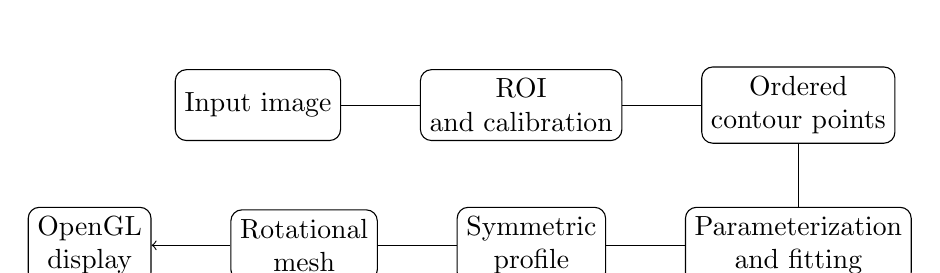
\begin{tikzpicture}[node distance=8mm and 10mm,
  every node/.style={draw,rounded corners,align=center,minimum height=9mm}]
\node (image) {Input image};
\node (roi) [right=of image] {ROI\\and calibration};
\node (points) [right=of roi] {Ordered\\contour points};
\node (fit) [below=of points] {Parameterization\\and fitting};
\node (sym) [left=of fit] {Symmetric\\profile};
\node (mesh) [left=of sym] {Rotational\\mesh};
\node (render) [left=of mesh] {OpenGL\\display};
\draw[->] (image)--(roi)--(points)--(fit)--(sym)--(mesh)--(render);
\end{tikzpicture}
\caption{Data flow of the reconstruction project}
\end{figure}

\section{Image Processing and Coordinate Calibration}

\subsection{ROI and threshold preview}
\texttt{extract\_vase.py} first selects a region of interest containing the vase
and coordinate grid.  The ROI is converted to grayscale and Gaussian filtered:
\[
I_g=G_\sigma * I.
\]
A threshold preview is then produced using
\[
B(u,v)=
\begin{cases}
255,& I_g(u,v)<T,\\
0,& I_g(u,v)\geq T.
\end{cases}
\]
The current implementation uses $T=100$.  This binary image is only a diagnostic
preview: automatically joining all dark pixels would incorrectly connect axes,
grid lines, text, and the vase boundary.

\figplaceholder[0.78\textwidth]{../threshold_preview.png}{Threshold preview}

\subsection{Pixel-to-coordinate transformation}

The user selects the origin $O$, a point at $x=5$, and a point at $y=5$.
If their pixel coordinates are
\[
O=(u_0,v_0),\quad X_5=(u_5,v_5),\quad Y_5=(u'_5,v'_5),
\]
the horizontal and vertical scales are
\[
s_x=\frac{u_5-u_0}{5},\qquad
s_y=\frac{v_0-v'_5}{5}.
\]
For a contour pixel $(u,v)$, the mathematical coordinate is
\[
x=\frac{u-u_0}{s_x},\qquad
y=\frac{v_0-v}{s_y}.
\]
The sign change in the second equation accounts for the fact that image rows
increase downward, whereas mathematical $y$ increases upward.

\subsection{Ordered contour points}

The contour points are recorded in boundary order rather than sorted by $x$.
This is important because vertical parts, horizontal parts, and folds near the
rim or base may cause several contour locations to have similar $x$ values.
The current input contains 84 non-repeated points after duplicate removal.

\figplaceholder[0.78\textwidth]{../contour_review.png}{Extracted contour review}

\section{Chord-Length Parameterization}

Let the ordered points be $\bm p_i=(x_i,y_i)$.  The chord increments and
normalized parameter are
\[
\Delta s_i=\|\bm p_i-\bm p_{i-1}\|_2,\qquad
s_i=\sum_{j=1}^{i}\Delta s_j,\qquad
t_i=\frac{s_i}{s_n}.
\]
The profile is represented parametrically as
\[
\bm r(t)=(x(t),y(t)),\qquad 0\leq t\leq 1.
\]
This avoids requiring $y$ to be a single-valued function of $x$ and gives
the parameter a geometric interpretation based on contour distance.

\section{Numerical Methods}

\subsection{Methods implemented in \texttt{fit\_methods.py}}

Each method independently interpolates or fits $x(t)$ and $y(t)$ and evaluates
the result at 1200 equally spaced parameter values.

\begin{enumerate}
\item \textbf{Linear interpolation}: local and stable, but only piecewise linear.
\item \textbf{Natural cubic spline}: globally smooth with zero second derivative
  at both endpoints, but susceptible to overshoot.
\item \textbf{PCHIP}: a shape-preserving cubic Hermite method that limits
  unnecessary extrema.
\item \textbf{Akima}: a local slope-based method that reduces the influence of
  abnormal neighboring slopes.
\item \textbf{Cubic B-spline interpolation}: smooth and exact at the data points,
  but sensitive to the global spline representation.
\item \textbf{Smoothing spline}: deliberately does not pass through every point;
  its smoothing parameter is $s=0.7462635893$ for the current data.
\item \textbf{Degree-five least-squares polynomial}: a global approximation used
  as a baseline, not as the final contour model.
\end{enumerate}

\subsection{Evaluation metrics}

The following quantities were computed from the same 84 input points.
For a method with predicted values $\widehat{\bm p}_i$ at the input parameters,
\[
e_i=\|\widehat{\bm p}_i-\bm p_i\|_2,\qquad
\mathrm{RMSE}_{\mathrm{train}}
=\sqrt{\frac{1}{n}\sum_{i=1}^{n}e_i^2}.
\]
For interpolation methods, the training error is expected to be zero and is
therefore not a useful selection criterion.  A more informative test is
leave-one-out cross-validation (LOOCV): remove one point, rebuild the method,
predict the removed point, and repeat for all 84 points.  The resulting
\[
\mathrm{RMSE}_{\mathrm{LOOCV}}
=\sqrt{\frac{1}{n}\sum_{i=1}^{n}e_{i,\mathrm{LOO}}^2}
\]
measures sensitivity to unseen points.

Two geometric diagnostics were also used:
\begin{itemize}
\item the arc length of the 1200-point fitted curve;
\item the percentage of evaluated points outside the bounding box of the input
  points, which detects overshoot.
\end{itemize}

\section{Numerical Comparison}

Table~\ref{tab:comparison} reports the computed results.  The full machine-readable
data are stored in the generated numerical-comparison CSV file in the
\texttt{fit\_output} directory.

\begin{table}[H]
\centering
\scriptsize
\caption{Numerical comparison of the seven fitting methods}
\label{tab:comparison}
\begin{tabular}{lrrrrr}
\toprule
\textbf{Method} &
\textbf{Train RMSE} &
\textbf{LOOCV RMSE} &
\textbf{LOOCV max} &
\textbf{Arc length} &
\textbf{Outside (\%)}\\
\midrule
Linear & 0.0000 & 0.0736 & 0.7610 & 34.1701 & 0.00\\
Natural cubic spline & 0.0000 & 0.0868 & 0.8534 & 34.9503 & 3.67\\
PCHIP & 0.0000 & 0.1051 & 2.6532 & 34.5964 & 0.00\\
Akima & 0.0000 & 0.0697 & 0.7675 & 34.7188 & 4.75\\
Cubic B-spline & 0.0000 & 0.3159 & 16.3930 & 35.0172 & 3.67\\
Smoothing spline & 0.1369 & 0.1655 & 1.4916 & 31.4478 & 2.00\\
Degree-five polynomial & 0.6298 & 0.6096 & 2.7325 & 27.5638 & 0.17\\
\bottomrule
\end{tabular}
\end{table}

\subsection{Interpretation}

The results support several numerical conclusions:
\begin{enumerate}
\item Linear interpolation has no overshoot and a moderate LOOCV error, but its
  derivative is discontinuous at every input point.
\item Akima has the lowest LOOCV RMSE, while its 4.75\% outside-box rate shows
  that local smoothness can still create small geometric excursions.
\item PCHIP is slightly less accurate under LOOCV than Akima, but it has no
  outside-box samples and preserves the contour's local shape.  This is valuable
  for a physical vase profile.
\item Natural cubic splines are smooth, but their 3.67\% outside-box rate
  confirms the possibility of overshoot near rapidly changing curvature.
\item Cubic B-splines have a substantially larger LOOCV error and extreme
  worst-case error.  Exact interpolation at the training points does not
  guarantee stable behavior between points.
\item The smoothing spline reduces the arc length and has nonzero training
  error, indicating visible smoothing bias.  It may be useful for noisy data,
  but it changes the measured geometry here.
\item The degree-five global polynomial has the largest training bias among the
  approximation methods and the shortest curve, so it cannot represent all
  local vase features simultaneously.
\end{enumerate}

\figplaceholder[0.91\textwidth]{../fit_output/method_comparison.png}{Right-half method comparison}
\figplaceholder[0.91\textwidth]{../fit_output/full_vase_comparison.png}{Full symmetric contour comparison}

\section{Geometry-Aware Final Fit}

The final program does not select one method blindly for the entire contour.
Instead, it uses geometric regions detected from the ordered data:
\begin{center}
\begin{tabular}{llll}
\toprule
\textbf{Region} & \textbf{Indices} & \textbf{Method} & \textbf{Reason}\\
\midrule
Top neck to base & 0--43 & PCHIP & preserve the narrow, monotone trend\\
Rounded base & 43--49 & Cubic spline & obtain a smooth rounded transition\\
Lower body & 49--56 & PCHIP & avoid unnecessary overshoot\\
Shoulder & 56--76 & Akima & handle local curvature changes\\
Rim and top & 76--83 & PCHIP & preserve the top transition\\
\bottomrule
\end{tabular}
\end{center}

Each segment fits both coordinates as functions of the same chord parameter.
The segment samples are joined without duplicate endpoints and resampled to a
uniform output grid.  The resulting final comparison figure is shown below.

\figplaceholder[0.91\textwidth]{../fit_output/final_fit_comparison.png}{Final piecewise fit and symmetric reconstruction}

\section{Symmetry and Three-Dimensional Reconstruction}

Assuming reflection symmetry about the $y$ axis, a right profile
\[
\bm r(t)=(x(t),y(t)),\qquad x(t)\geq 0
\]
is mirrored by
\[
\mathcal M(x,y)=(-x,y).
\]
The full two-dimensional contour is formed by concatenating the reversed
mirrored side with the original right side:
\[
\bm r_{\mathrm{full}}=
\left\{(-x(1-t),y(1-t))\right\}
\cup
\left\{(x(t),y(t))\right\}.
\]

The OpenGL renderer uses the right curve as a surface of revolution:
\[
\bm S(t,\theta)=
\bigl(x(t)\cos\theta,\ y(t),\ x(t)\sin\theta\bigr),
\qquad 0\leq\theta<2\pi.
\]
The current implementation uses 96 angular slices.  Adjacent profile samples
and angular samples form quadrilateral strips.  The program also computes
approximate normals, depth testing, lighting, wireframe mode, camera movement,
and interactive rotation.

\section{Reproducibility}

\subsection{Python processing}
\begin{lstlisting}[language=Python]
python -m pip install -r requirements.txt
python extract_vase.py
python fit_methods.py
python final_fit.py
\end{lstlisting}

\subsection{OpenGL build}
\begin{lstlisting}
cd viewer
cmake -S . -B build
cmake --build build --config Release
VaseReconstruction.exe ../../fit_output/final_fit_right_curve.csv
\end{lstlisting}

\section{Conclusion}

The project demonstrates that contour reconstruction is not only a plotting
problem.  Parameter choice, interpolation stability, shape preservation, and
validation all affect the final geometry.  The numerical comparison shows why
training-point error alone is misleading for interpolants.  LOOCV exposes the
instability of the cubic B-spline and the bias of the polynomial and smoothing
fits, while geometric diagnostics reveal overshoot that an error norm alone may
not show.

For this data, a piecewise strategy is more appropriate than a single global
method: PCHIP provides shape preservation in the main body, a local cubic spline
smooths the rounded base, and Akima handles the shoulder.  The final profile can
then be mirrored and rotated into a stable, interpretable three-dimensional
vase.

\end{document}
